\documentclass[a4paper]{article}
\usepackage[latin1]{inputenc}
\usepackage[brazil]{babel}
\usepackage[normalem]{ulem}
\usepackage[dvips]{graphicx}
\usepackage{longtable}
%\usepackage{html}
\usepackage{hyperref}
\usepackage{enumerate}
\usepackage{setspace}
\usepackage{float}      
\usepackage{fancyvrb}
\usepackage{boxit}
\usepackage{graphicx}
\usepackage{makeidx,shortvrb,latexsym}

%===== C�digos Fonte =====
\newenvironment{codeverbatim}{\VerbatimEnvironment \small
   \begin{Verbatim}[xleftmargin=20mm]}
   {\end{Verbatim}}
%=======
\floatstyle{plain}  % tipos: plain, boxed, ruled
\newfloat{codigo}{tbp}{lop}[section]  % numera os captions com  n�mero de se��o.
\floatname{codigo}{Listagem}
% nome para ser usado no sum�rio
\newcommand{\listofcodename}{Lista de C�digos}
%=========================

\def\version{1.0.0}
\def\stableversion{3.2} 

\title{
	SMS Box V1.01 \\ Guia do usu�rio \\
	\small {vers�o \version}
}
\author{Rafael Dias Menezes}
\date{Fev/2010}


\begin{document}
\onehalfspacing
%\maketitle


\ifpdf
  \pdfbookmark{Title Page}{title}
\fi
\newlength{\centeroffset}
\setlength{\centeroffset}{-0.5\oddsidemargin}
\addtolength{\centeroffset}{0.5\evensidemargin}
%\addtolength{\textwidth}{-\centeroffset}
\thispagestyle{empty}
\vspace*{\stretch{1}}
\noindent\hspace*{\centeroffset}\makebox[0pt][l]{\begin{minipage}{\textwidth}
\flushright
{\Huge\bfseries Manual de Opera��o \\ 
SMS Box
}

\noindent\rule[-1ex]{\textwidth}{5pt}\\[2.5ex]
\hfill\emph{}
\end{minipage}}

\vspace{\stretch{1}}
\noindent\hspace*{\centeroffset}\makebox[0pt][l]{\begin{minipage}{\textwidth}
\flushright
{\bfseries 
  Rafael Dias Menezes\\[1.5ex]
} 
Vers�o~1.00 \\ mar�o/2010
\end{minipage}}

%\addtolength{\textwidth}{\centeroffset}
\vspace{\stretch{2}}


%\pagebreak
%\begin{small} 
%  Copyright \copyright 1995-2005 Tobias Oetiker and Contributers.  Todos os direitos reservados.
 
%  This document is free; you can redistribute it and/or modify it
%  under the terms of the GNU General Public License as published by
%  the Free Software Foundation; either version 2 of the License, or
%  (at your option) any later version.
%  
%  This document is distributed in the hope that it will be useful, but
%  WITHOUT ANY WARRANTY; without even the implied warranty of
%  MERCHANTABILITY or FITNESS FOR A PARTICULAR PURPOSE\@.  See the GNU
%  General Public License for more details.
  
%  You should have received a copy of the GNU General Public License
%  along with this document; if not, write to the Free Software
%  Foundation, Inc., 675 Mass Ave, Cambridge, MA 02139, USA.

%\end{small}


\endinput

%

% Local Variables:
% TeX-master: "lshort2e"
% mode: latex
% mode: flyspell
% End:

\typeout{Copyright Rafael Dias @ Taioba Corporation}
\tableofcontents
\listoffigures
\listoftables
%%%%%%%%%%%%%%%%%%%%%%%%%%%%%%%%%%%%%%%%%%%%%%%%%%%%%%%%%%%%%%%%%%%%%%%%%%%%%%%%%%%%%%%%%%%%%%%    

\section{Overview}
  
  A plataforma SMS Box permite o envio de mensagens de texto (SMS) atrav�s de uma plataforma 
  de hardware baseada em um processador de 8 bits controlando um modem GSM.

  Este guia foca na utiliza��o do SMS Box como uma plataforma de envio de SMS integrada com a aplica��o GSMComando e a sua integra��o no VosCenter.
    
  \subsection{Placa SMS Box}
    A placa � composta pelos seguintes componentes:
    
    \begin{itemize}
      \item Microcontrolador de uso geral PIC18LF4680 I/P;
      \item Mem�ria flash SDRAM AT45DB041 para download de firmware e gera��o de logs;
      \item Circuito de l�gica de apoio, composta de portas l�gicas e multiplexadores que s�o encarregados 
            de realizar a troca dos chips e conforma��o dos n�veis el�tricos entre o microcontrolador e o modem GSM;
      \item Modem GSM SIMCOM 340C;
      \item LEDs de status de opera��o da m�quina; 
      \item LED de status de conex�o do modem GSM;
      \item Soquetes de SIM Cards; 
      \item Conector de comunica��o serial com PC \textit{Host}; 
      \item Conector de debug do modem GSM.
    \end{itemize}
    
%%%%%%%%%%%%%%%%%%%%%%%%%%%%%%%%%%%%%%%%%%%%%%%%%%%%%%%%%%%%%%%%%%%%%%%%%%%%%%%%%%%%%%%%%%%%%%%    

\section{Utiliza��o da SMS Box}

\subsection{Requisitos}
Para utilizar a SMS Box os seguintes �tens se faz necess�rios:
    \begin{itemize}
      \item SMS Box;
      \item Fonte de alimenta��o AC/DC (7.5Vdc � 15Vdc @ 0,4A), 2.5mm;
      \item Cabos para comunica��o entre a SMS Box e o PC \textit{Host}.
    \end{itemize}


\subsection{Layout}
  A figura \ref{fig:laySMSBOX_top} mostra a disposi��o dos componentes constituintes da SMS Box V1.01.
  
\begin{figure}[!htb]
  \centering
  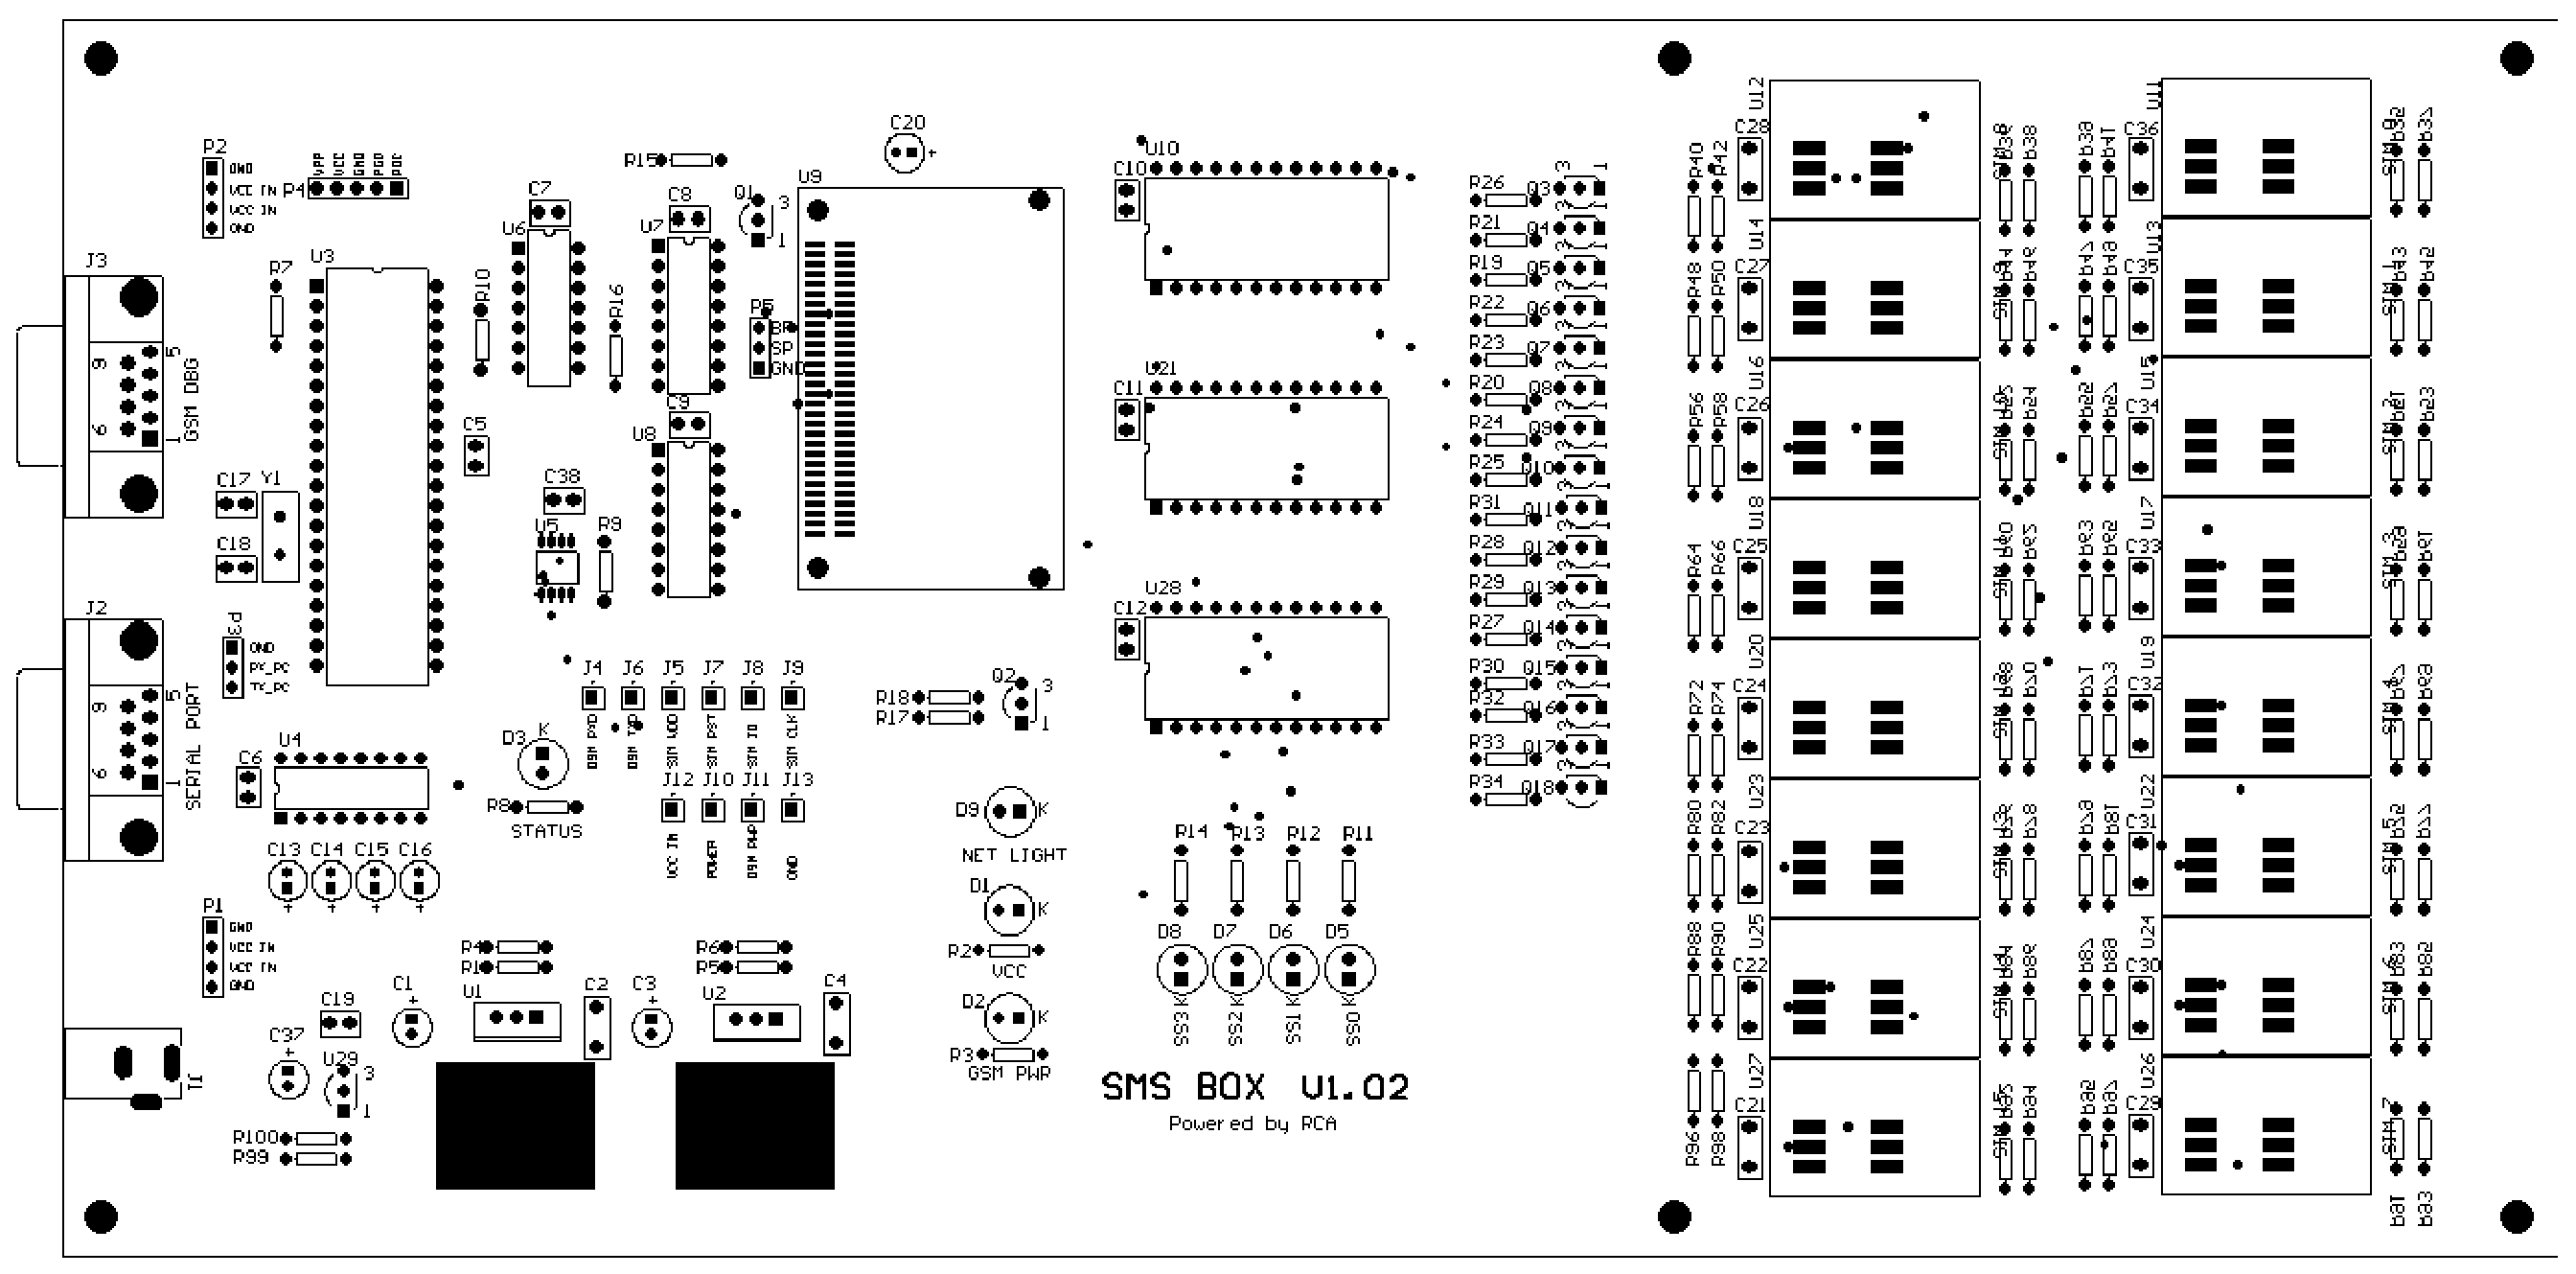
\includegraphics[scale=.3]{Layout.eps}
  \caption{Layout SMS Box - Top View}
  \label{fig:laySMSBOX_top}
\end{figure}
  
  
  
\subsection{Energiza��o}
A SMS Box requer uma alimenta��o de 7.5Vdc � 15Vdc. A liga��o deve 
ser realizada atrav�s do jack J1. Para alimenta��o de diversas SMS Box 
aproveitando a mesma fonte devemos utilizar um \textit{flat cable} 
interconectando as placas atrav�s das barras de terminais P1 e P2.


\subsection{Configurando a SMS Box}
  Antes de energizar a placa verifique se todos os componentes est�o 
devidamente conectados, bem como se o jumper P5 est� conectado entre 
os pontos \textbf{SP} e \textbf{GND}.  Sem a presen�a dessa conex�o a SMS Box n�o funcionar�.

  A comunica��o entre a SMS Box e o \textit{Host} � realizado atrav�s de um link de comunica��o serial RS232 
com \textit{baudrate} fixo em 19200bps. Esse par�metro � muito importante para a conex�o da mesma com o 
\textit{software} de controle, ou seja, o \textit{GSMComando} ou a pr�pria \textit{Switch}. 

Assim que a SMS Box � energizada, o LED \textit{NET LIGHT} come�a a piscar interruptamente indicando que o modem GSM est� em opera��o. 
A tabela \ref{tab:PadraoNET_LIGHT} mostra o estado apresentado pelo padr�o de piscadas do LED \textit{NET LIGHT}.

	\begin{table}[!htb]
		\centering
		\begin{tabular}{|c|p{4.5cm}|}
			\hline
			\textbf{Estado NET LIGHT}			        &  		\multicolumn{1}{|c|}{\textbf{fun��o no SIM340C}} \\ \hline 
			Desligado                             & SIM340C n�o est� ligado       \\ \hline
      64ms ligado / 800ms + 50\% desligado  & SIM340C n�o encontrou a rede  \\ \hline
      64ms ligado / 3000ms + 50\% desligado & SIM340C encontrou a rede      \\ \hline
		\end{tabular}
		\label{tab:PadraoNET_LIGHT}
		\caption{Estado de opera��o do LED NET LIGHT}
	\end{table}
  

Adicionalmente ao LED NET LIGHT h� o LED STATUS que indica o estado de opera��o da SMS Box com o \textit{Host} e alguns estados de erro na plataforma. 
Esses estados s�o dados pela tabela \ref{tab:PadraoSTATUS}.

	\begin{table}[!htb]
		\centering
		\begin{tabular}{|c|p{4.5cm}|}
			\hline
			\textbf{Estado LED STATUS}			              &  		\multicolumn{1}{|c|}{\textbf{estado SMS Box}}     \\ \hline 
			Desligado                                     &  SMS Box desligado                                    \\ \hline
			Uma piscada de 10ms e 2990ms desligado        &  SMS Box ligado e sem conex�o com o \textit{Host}     \\ \hline
			Duas piscadas de 10ms e 2970ms desligado      &  SMS Box ligado e com conex�o com o \textit{Host}     \\ \hline
		\end{tabular}
		\label{tab:PadraoSTATUS}
		\caption{Estado de opera��o do LED STATUS}
	\end{table}

%%%%%%%%%%%%%%%%%%%%%%%%%%%%%%%%%%%
  
\subsection{Utilizando a SMS Box com a aplica��o GSMComando}
  \subsubsection{Introdu��o}
  Para a realiza��o de testes com a SMS Box podemos utilizar uma aplica��o chamada GSMComando, que tem por fun��o principal 
realizar o controle da SMS Box. Esse controle � realizado atrav�s da troca de mensagens entre o GSMComando e a SMS Box. O requisito 
mandat�rio para a opera��o da plataforma � a presen�a de um canal de comunica��o serial DB9. Nos computadores atuais a interface 
de comunica��o \textit{COM} n�o � mais fornecida, sendo necess�rio adquirir placas de expans�o para interface serial ou conversores USB/RS232.

  \subsubsection{Fun��es b�sicas}
Assim que a aplica��o GSMComando � executada, este apresenta a tela mostrada na figura \ref{fig:GSMComando_telainicial}.

    \begin{figure}[!htb]
      \centering
      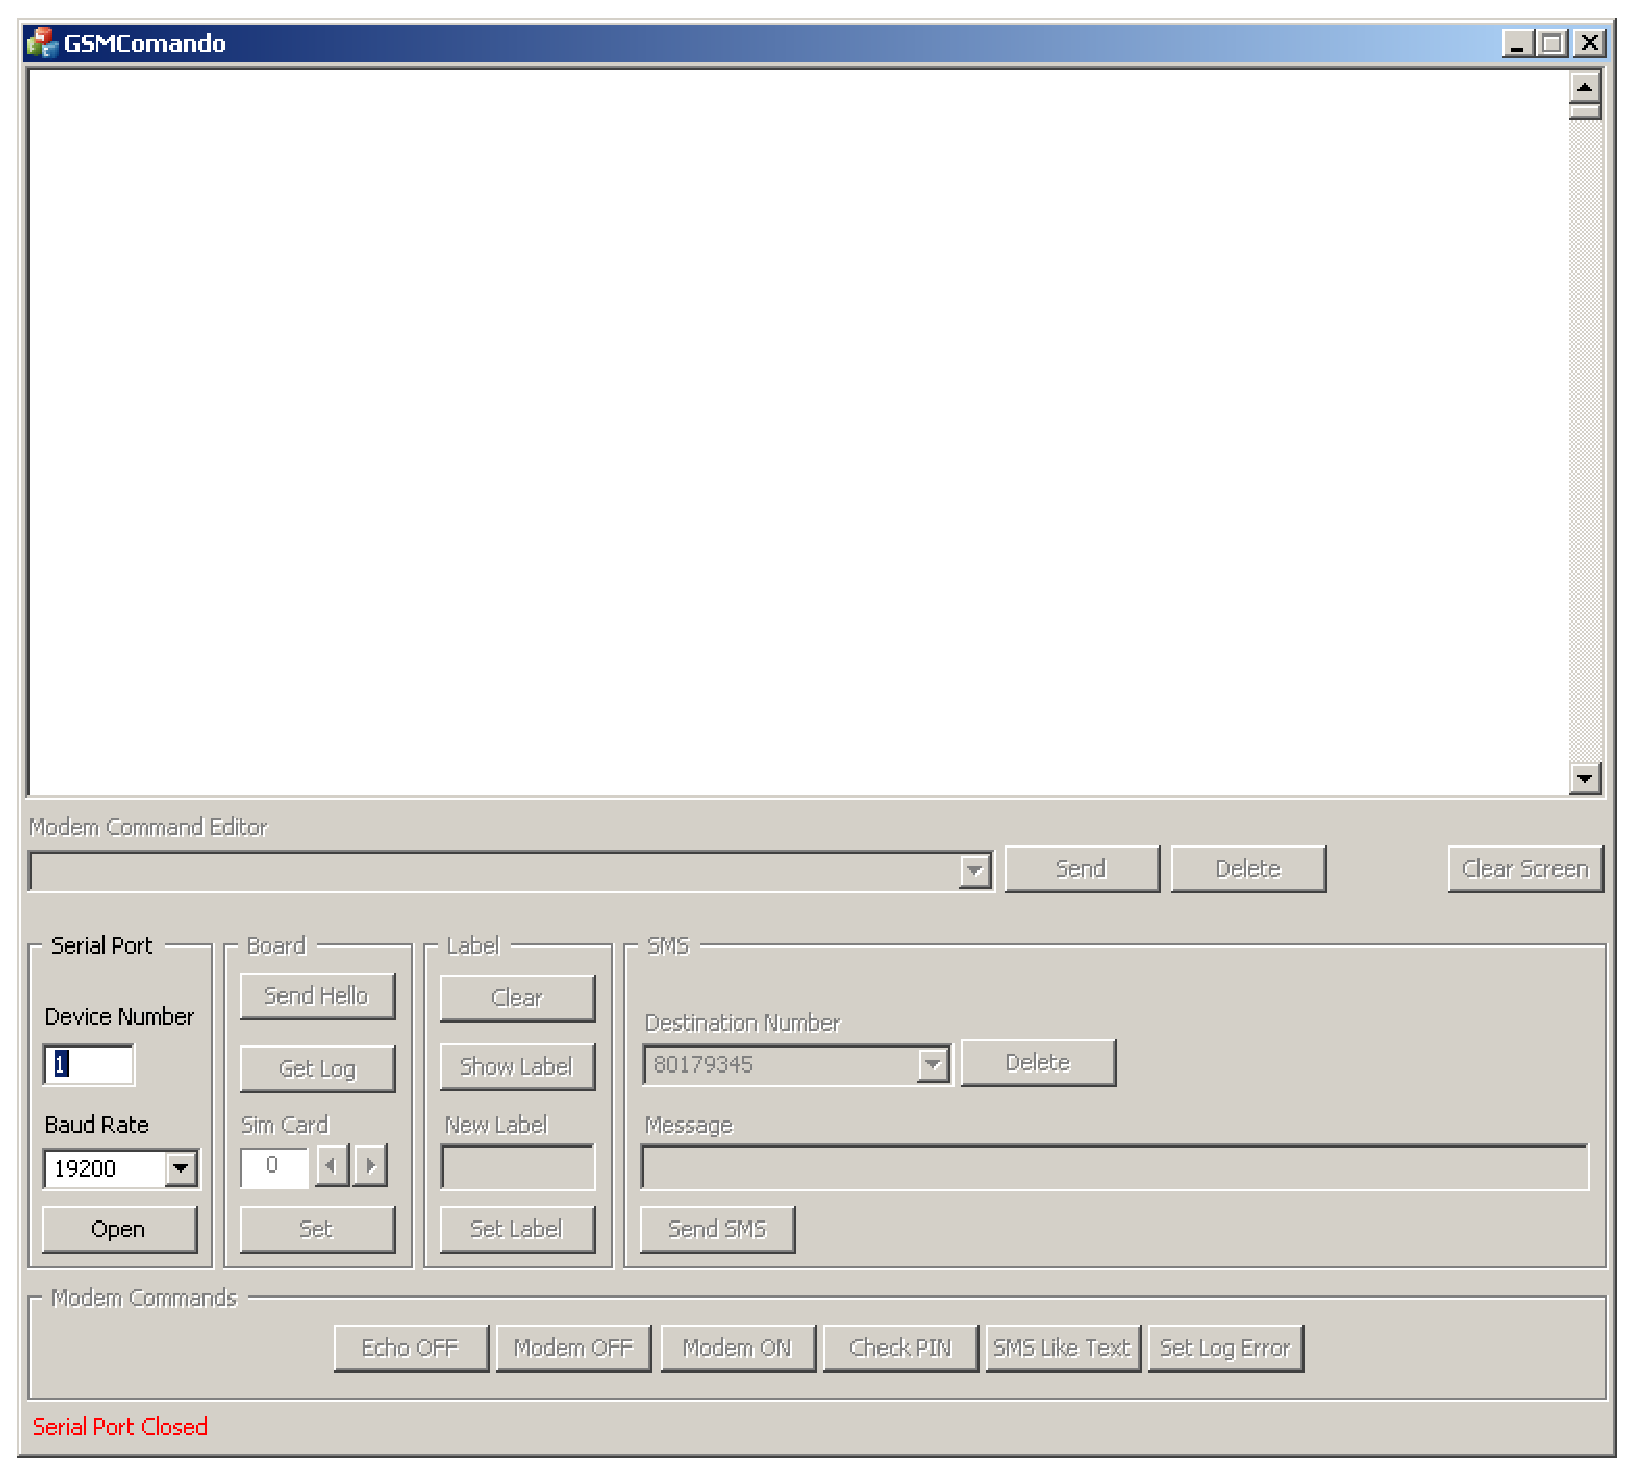
\includegraphics[scale=.35]{GSMComando.Telainicial.eps}
      \caption{Tela inicial GSMComando}
      \label{fig:GSMComando_telainicial}
    \end{figure}
  
  Para que a comunica��o entre a SMS Box e o GSMComando seja estabelecida com sucesso deve-se
inicialmente configurar a porta de comunica��o serial atrav�s dos campos \textbf{Device Number} e \textbf{Baud Rate}, 
localizados no lado inferior esquedo da aplica��o. Caso a porta configurada esteja errada, assim que houver uma 
tentativa de abrir a porta serial a aplica��o mostrar� na barra de status a mensagem de erro \textbf{\textit{Error openning COMX}}. 
Como informado anteriormente, o baudrate utilizado pela SMS Box � fixo em 19200bps e a utiliza��o de um baudrate diferente deste 
acarreta no n�o estabelecimento da comunica��o entre o \textit{Host} e a SMS Box. 

  Ap�s abrir a porta de comunica��o serial os bot�es de controle da aplica��o s�o habilitados e podemos operar a SMS Box. 
A tabela  \ref{gsmcomando:botoes_funcionalidades} descreve os controles e suas funcionalidades.

\begin{center}
\begin{longtable}{|l|p{7.5cm}|}

\hline \multicolumn{1}{|c|}{\textbf{Bot�o}} & \multicolumn{1}{c|}{\textbf{Funcionalidade}} \\[0.5ex] \hline 
\endfirsthead

\multicolumn{2}{c}%
{{\bfseries \tablename\ \thetable{} -- continua��o da p�gina anterior}} \\
\hline \multicolumn{1}{|c|}{\textbf{Bot�o}} & \multicolumn{1}{c|}{\textbf{Funcionalidade}} \\[0.5ex] \hline 
\endhead

\hline \multicolumn{2}{|r|}{{Continua na pr�xima p�gina}} \\[0.5ex] \hline
\endfoot

\endlastfoot
%%%%%%%%%%%%%%%%%%%%%%%%%%%%%%%%%%%%%%%%%%%%%%%%%%%%%%%%%%%%%%%%%%%%%%%%%%%%%%%%%%%%%%%%%%%%%%%%%%%%%%%%%%%%%%%%
\textit{Open}             & Realiza a abertura/fechamento da porta de comunica��o serial          \\ \hline
%%%%%%%%%%%%%%%%%%%%%%%%%%%%%%%%%%%%%%%%%%%%%%%%%%%%%%%%%%%%%%%%%%%%%%%%%%%%%%%%%%%%%%%%%%%%%%%%%%%%%%%%%%%%%%%%
\textit{Baud Rate}        & Configura o baud rate da comunica��o entre a SMS Box e o GSMComando   \\ \hline
%%%%%%%%%%%%%%%%%%%%%%%%%%%%%%%%%%%%%%%%%%%%%%%%%%%%%%%%%%%%%%%%%%%%%%%%%%%%%%%%%%%%%%%%%%%%%%%%%%%%%%%%%%%%%%%%
\textit{Device Number}    & Indica qual � a placa que ser� acessada.                               \\ \hline    
%%%%%%%%%%%%%%%%%%%%%%%%%%%%%%%%%%%%%%%%%%%%%%%%%%%%%%%%%%%%%%%%%%%%%%%%%%%%%%%%%%%%%%%%%%%%%%%%%%%%%%%%%%%%%%%%                   
\textit{Send Hello}       & Envia mensagem de in�cio de comunica��o entre a SMS Box e o GSMComando. 
                            O envio deste comando � mandat�rio na opera��o da SMS Box.                  \\ \hline                       
%%%%%%%%%%%%%%%%%%%%%%%%%%%%%%%%%%%%%%%%%%%%%%%%%%%%%%%%%%%%%%%%%%%%%%%%%%%%%%%%%%%%%%%%%%%%%%%%%%%%%%%%%%%%%%%%
\textit{Get Log}          & Envia mensagem de solicita��o de captura de Log. Assim que a linha 
                            de log � recebido pela aplica��o GSMComando, o mesmo � adicionado no 
                            final do arquivo de log modem.txt.                                          \\ \hline     
%%%%%%%%%%%%%%%%%%%%%%%%%%%%%%%%%%%%%%%%%%%%%%%%%%%%%%%%%%%%%%%%%%%%%%%%%%%%%%%%%%%%%%%%%%%%%%%%%%%%%%%%%%%%%%%%                            
\textit{Set Sim Card}     & Controle \textbf{Sim Card} e o bot�o \textbf{Set} trabalham em conjunto 
                            para escolher qual SIM Card deve estar operante no momento. Na SMS Box, os LEDs SS0 � SS3 
                            indicam qual Sim Card est� ativo no momento.                                \\ \hline
%%%%%%%%%%%%%%%%%%%%%%%%%%%%%%%%%%%%%%%%%%%%%%%%%%%%%%%%%%%%%%%%%%%%%%%%%%%%%%%%%%%%%%%%%%%%%%%%%%%%%%%%%%%%%%%%
\textit{Clear}            & Ap�s realizar a leitura do r�tulo do Sim Card, podemos limp�-lo atrav�s deste bot�o. 
                            A leitura do r�tulo do Sim card s� pode ser realizada quando o modem se registrar na rede 
                            utilizando o Sim Card.                                                      \\ \hline
%%%%%%%%%%%%%%%%%%%%%%%%%%%%%%%%%%%%%%%%%%%%%%%%%%%%%%%%%%%%%%%%%%%%%%%%%%%%%%%%%%%%%%%%%%%%%%%%%%%%%%%%%%%%%%%%
\textit{Show Label}       & Realiza a leitura do r�tulo do Sim Card. A leitura do r�tulo do Sim card somente 
                            pode ser realizada quando o modem se registrar na rede utilizando o Sim Card. \\ \hline
%%%%%%%%%%%%%%%%%%%%%%%%%%%%%%%%%%%%%%%%%%%%%%%%%%%%%%%%%%%%%%%%%%%%%%%%%%%%%%%%%%%%%%%%%%%%%%%%%%%%%%%%%%%%%%%%
\textit{Set Label}        & Realiza a leitura do r�tulo do Sim Card. A leitura do r�tulo do Sim card s� 
                            pode ser realizada quando o modem se registrar na rede utilizando o Sim Card. \\ \hline
%%%%%%%%%%%%%%%%%%%%%%%%%%%%%%%%%%%%%%%%%%%%%%%%%%%%%%%%%%%%%%%%%%%%%%%%%%%%%%%%%%%%%%%%%%%%%%%%%%%%%%%%%%%%%%%%
\textit{SMS}              & Controles respons�veis pelo envio de mensagens SMS pelo SMS Box. At� a vers�o 1.02 do 
                            SMS Box os SMSs podem ser enviados somente com o modo texto.                  \\ \hline
%%%%%%%%%%%%%%%%%%%%%%%%%%%%%%%%%%%%%%%%%%%%%%%%%%%%%%%%%%%%%%%%%%%%%%%%%%%%%%%%%%%%%%%%%%%%%%%%%%%%%%%%%%%%%%%%                            
\textit{Modem commands}   & Lista diversos controles utilizados para enviar comandos AT pr�-formatados ao modem. 
                            Entre as op��es existentes temos comandos para desligar e ligar o m�dulo RF do modem GSM, 
                            desligar o echo, checar se o SIM Card est� conectado (sem a necessidade de esperar o modem 
                            responder com um \textit{Call Ready}), SMS modo texto e setar visualiza��o de erro. 
                            Apresenta tamb�m  a op��o de enviar comandos AT editados pelo usu�rio atrav�s do controle 
                            \textit{Modem Command Editor}, logo abaixo do controle memo que mostra a troca de mensagens
                            entre a SMS Box e o GSMComando.                                               \\ \hline
%%%%%%%%%%%%%%%%%%%%%%%%%%%%%%%%%%%%%%%%%%%%%%%%%%%%%%%%%%%%%%%%%%%%%%%%%%%%%%%%%%%%%%%%%%%%%%%%%%%%%%%%%%%%%%%%                            
\caption{GSMComando, bot�es e funcionalidades.} 
\label{gsmcomando:botoes_funcionalidades} 

\end{longtable}
\end{center}


\subsubsection{Opera��o}

  Vamos dar em forma de pequenos passos como deve ser realizado a opera��o da SMS Box com o GSMComando:
  \begin{enumerate}[i.]
    \item Energize a SMS Box. Neste momento os LEDs SSx devem permanecer ligados e o LED NetLight iniciar a 
          piscar. Depois de um tempo o LED Status inicia a piscar indicando que o modem est� no operante e que 
          o \textit{Host} n�o est� comunicando com a SMS Box;
    \item Conecte o link de comunica��o serial;
    \item Execute a aplica��o GSMComando e realize a configura��o b�sica da aplica��o, como o baudrate, porta de comunica��o, etc;
    \item Abra a porta de comunica��o serial, atrav�s do bot�o \textit{Open};
    \item Inicie a comunica��o com a SMS Box enviando um comando HELLO. A partir deste momento o LED Status alterna entre 
          representa��o do estado de opera��o do modem e o estado de conectividade do \textit{Host};
    \item Envie os comandos \textit{Echo Off}, \textit{Modem Off}, \textit{SMS Like Text} e \textit{Set Log Error}. A ordem de envio n�o � mandat�rio. 
          Os comandos enviados e as respostas recebidas pela aplica��o GSMComando s�o logadas na parte superior da aplica��o, sendo que as linhas brancas 
          s�o os comandos enviados e as linhas azuis s�o as respostas recebidas;
    \item Certifique-se de que h� pelo menos um SIM Card inserido na SMS Box;
    \item Escolha o Sim Card desejado, atrav�s dos controles \textit{Sim Card} e \textit{Set}. Neste momento aparecer� a mensagem ACTIVE SIM CARD na
          parte superior da aplica��o; 
    \item Espere pelo recebimento da mensagem \textit{Call Ready}. A partir do momento da recep��o desta mensagem a SMS Box estar� apta a enviar SMSs, 
          obter o label do SIM Card e realizar todas as demais opera��es. 
  \end{enumerate}
  
  
%%%%%%%%%%%%%%%%%%%%%%%%%%%%%%%%%%%%%%%%%%%%%%%%%%%%%%%%%%%%%%%%%%%%%%%%%%%%%%%%%%%%%%%%%%%%%%%%%%

\subsection{Integrando a SMS Box ao VosCenter}
  Para integrar a SMS Box ao VosCenter devemos inicialmente verificar se o script LUA que 
utilizado para realizar a opera��o fora implementado para operar com as placas Khomp. Essa configura��o 
da plataforma � muito importante pois o script LUA para a SMS Box � diferente do script LUA que funciona com as placas Khomp. 
O motivo � que as placas Khomp funcionam somente com 1 Sim card por modem e o SMSBOX funciona com at� 16 e implementa a fun��o NEXT SIMCARD.
Para o funcionamento das suas placas simultaneamente na mesma m�quina, configurar para a placa Khomp o 
script 1001 e para a placa SMSBOX o script 9999.

\subsubsection{Instala��o das placas no ambiente VosCenter}

  Roteiro executado SMSBOX \\
  
  \begin{center}
    \begin{minipage}[!htb]{6cm}
      SERVER:NETSMSBD \\
      DATABASE:Voscenter2 \\
      USER:switch \\
      PASSWORD:******** \\
    \end{minipage}
  \end{center}

  ECS 
  
  \begin{center}
    \begin{minipage}[!htb]{6cm}
      URL:http://netsmsbd:8080/ECS/Controller \\
      USER: placarca \\
      PASSWORD: ******** \\
    \end{minipage}
  \end{center}

  A vers�o da Switch � a 7.17.0.0, espec�fica sem prote��o.

  Na listagem \ref{code:config.xml} mostramos a configura��o para a placa SMS Box e Khomp.

  \begin{codigo}[!htb]
     \tiny  % tamanho da fonte
     \begin{boxit}  % coloca o c�digo dentro de um Box
        \vspace{2mm}
        \VerbatimInput[xleftmargin=8mm,numbers=left,obeytabs=true]{config.xml}
     \end{boxit}
     \caption{Arquivo config.xml do script SMSBOX.}
     \label{code:config.xml}
  \end{codigo}

    
    Na configura��o da tabela \textit{TCTIport}, muito importante observar dois campos: \textit{SerialPortNumber} e 
  \textit{SerialPortBaudrate}. Para a SMS Box, � necess�rio configurar os dois.

  � importante configurar na tabela T\_ICP\_SMS\_CONFIGURATION o campo NU\_TIME\_DELAY para 20. Isso quer dizer 
  que entre uma mensagem e outra, o sistema colocar� um delay de 20seg. Para as placas SMSBOX, este tempo 
  � necess�rio para n�o gerar congestionamento na rede.Talvez seja poss�vel colocar um n�mero menor, por exemplo 13.

\subsubsection{Roteiro de teste - VosCenter / SMSBOX}
  Para a correta verifica��o do fncionamento da SMS Box com o VosCenter, siga o procedimentio descrito abaixo:
  
  \begin{enumerate}
    \item Verifique se as placas est�o em opera��o.
        Ap�s realizar o \textit{upload} do firmware para a placa, verifique o 
          funcionamento observando os LEDs STATUS e NET LIGHT, como descrito nas tabelas \ref{tab:PadraoNET_LIGHT} e \ref{tab:PadraoSTATUS}.
          Se o LED n�o estiver piscando, a placa est� com algum problema de inicializa��o do firmware.

    \item Realize testes b�sico de comunica��o entre servidor e a SMS Box. Para testar a comunica��o entre 
        o servidor e a placa, mandar mensagens, passar por todos os chips, etc. Esta etapa pode ser realizada com o GSMComando. 
        
    \item Enviar mensagem para um determinado grupo. Inicie um script LUA 
        (j� existente na m�quina \textit{SMSBOXSW01}) na porta e verificar o \textbf{idClient} configurado no XML.

    \item Responda a mensagem enviada pela plataforma e verifique se o conte�do foi gravado na base de dados.
        
    \item Extraia o relat�rio a partir do ECS e verifique se as mensagens enviadas batem com o relat�rio. Todas as mensagens 
          enviadas devem bater no relat�rio gerencial e anal�tico do ECS.
        
    \item Verifique ciclo de envio das mensagens
        \begin{enumerate}[a.]
          \item Esgotar as mensagens em todos os chips;
          \item Verificar se a aplica��o altera de um sim card para outro automaticamente;
          \item Verificar se ap�s o sim card 16, a aplica��o muda para o sim card  1 automaticamente.
        \end{enumerate}
    
    \item Verifique se a procedure SP\_EXPORT\_DATA est� retornando os dados corretamente
    
  \end{enumerate}


%%%%%%%%%%%%%%%%%%%%%%%%%%%%%%%%%%%%%%%%%%%%%%%%%%%%%%%%%%%%%%%%%%%%%%%%%%%%%%%%%%%%%%%%%%%%%%%%%%
  
 
\subsubsection{Resolu��o de problemas}
  Os principais problemas que enfrentamos na opera��o da SMS Box s�o decorrentes da mal instala��o dos Sim cards e configura��o 
errada do baud rate e canal de comunica��o. Durante a opera��o do mesmo, pode ocorrer do modem cessar o envio de respostas aos comandos AT e 
nesta ocasi�o somente nos resta a op��o de desligar e ligar o modem.


\clearpage
\pagestyle{plain}
\end{document}
